\begin{center}
  \section{\capitalisewords{Role of ISRO in Technological Advancement}}
  Suprio Dutta, 3$^{rd}$ Year, ECE
\end{center}

\setcounter{figure}{0}

\begingroup
\makeatletter
\renewcommand\subsection{\@startsection{subsection}{2}{\z@}%
  {1.2ex}{0.6ex}{\normalfont\large\bfseries}}
\makeatother
\begin{multicols}{2}
  \begin{abstract}
    \bfseries
    ISRO viz Indian Space Research Organisation established in 1969 was never solely about rockets[1]. From the
    beginning it mainly focused on solving practical problems such as delivering weather data to coastal fishermen,
    emergency communication after disaster and providing healthcare and education to remote and inaccessible
    villages. This thinking carried into the missions as well. Chandrayaan-1[2] confirmed water molecules on the
    lunar surface, reshaping international lunar science. Mangalyaan reached Mars orbit on its first attempt and did
    so at a cost almost half of the Interstellar movie. This is because, India had access to limited resource and financial
    support as a result engineers had to figure how to stretch out every rupee. Aditya-L1[3], now stationed at the L1
    Lagrange point[4], gives India a route to heliophysics[5], a domain only few agencies currently have access to.
    Most Indian don’t realise we have our own GPS which is NavIC[6] which became one of our greatest asset during
    Operation Sindoor. ISRO satellites are keeping education and telemedicine running in areas where roads and
    electricity are still unreliable. ISRO isn’t operating alone anymore. Private players like Skyroot[7] and Agnikul[8],
    alongside academic partnerships, are developing so rapidly that it’s difficult for a single government agency to
    manage alone. Gaganyaan[9] India's first crewed mission is the most important upcoming project. If it succeeds
    India will be the fourth country to send human to space.
  \end{abstract}

  \subsection*{\centering\uppercase{INTRODUCTION}}
  Space technology plays an important role in day-to-day life. Services such as communication,
  navigation, weather forecasting, disaster warnings and every small services relies heavily on satellites.
  For India, this infrastructure wasn’t borrowed from anyone. Much of it is developed from indigenous
  efforts and homegrown technology.
  ISRO was established in 1969 under Dr. Vikram Sarabhai[10], a scientist who believed, that space
  technology should serve people. That mindset to serve is relevant even today. In its early years, ISRO
  operated on tight budgets and limited access to foreign technology, Despite the scarcity and threat of
  foreign sanction ISRO continued to build its own satellites and launch vehicles rather than depend on
  others. This costed much more time but gave self-reliance in comparison to other agencies.

  \begin{center}
\vspace{-0.5em}
\begin{minipage}{0.98\columnwidth}
\centering
    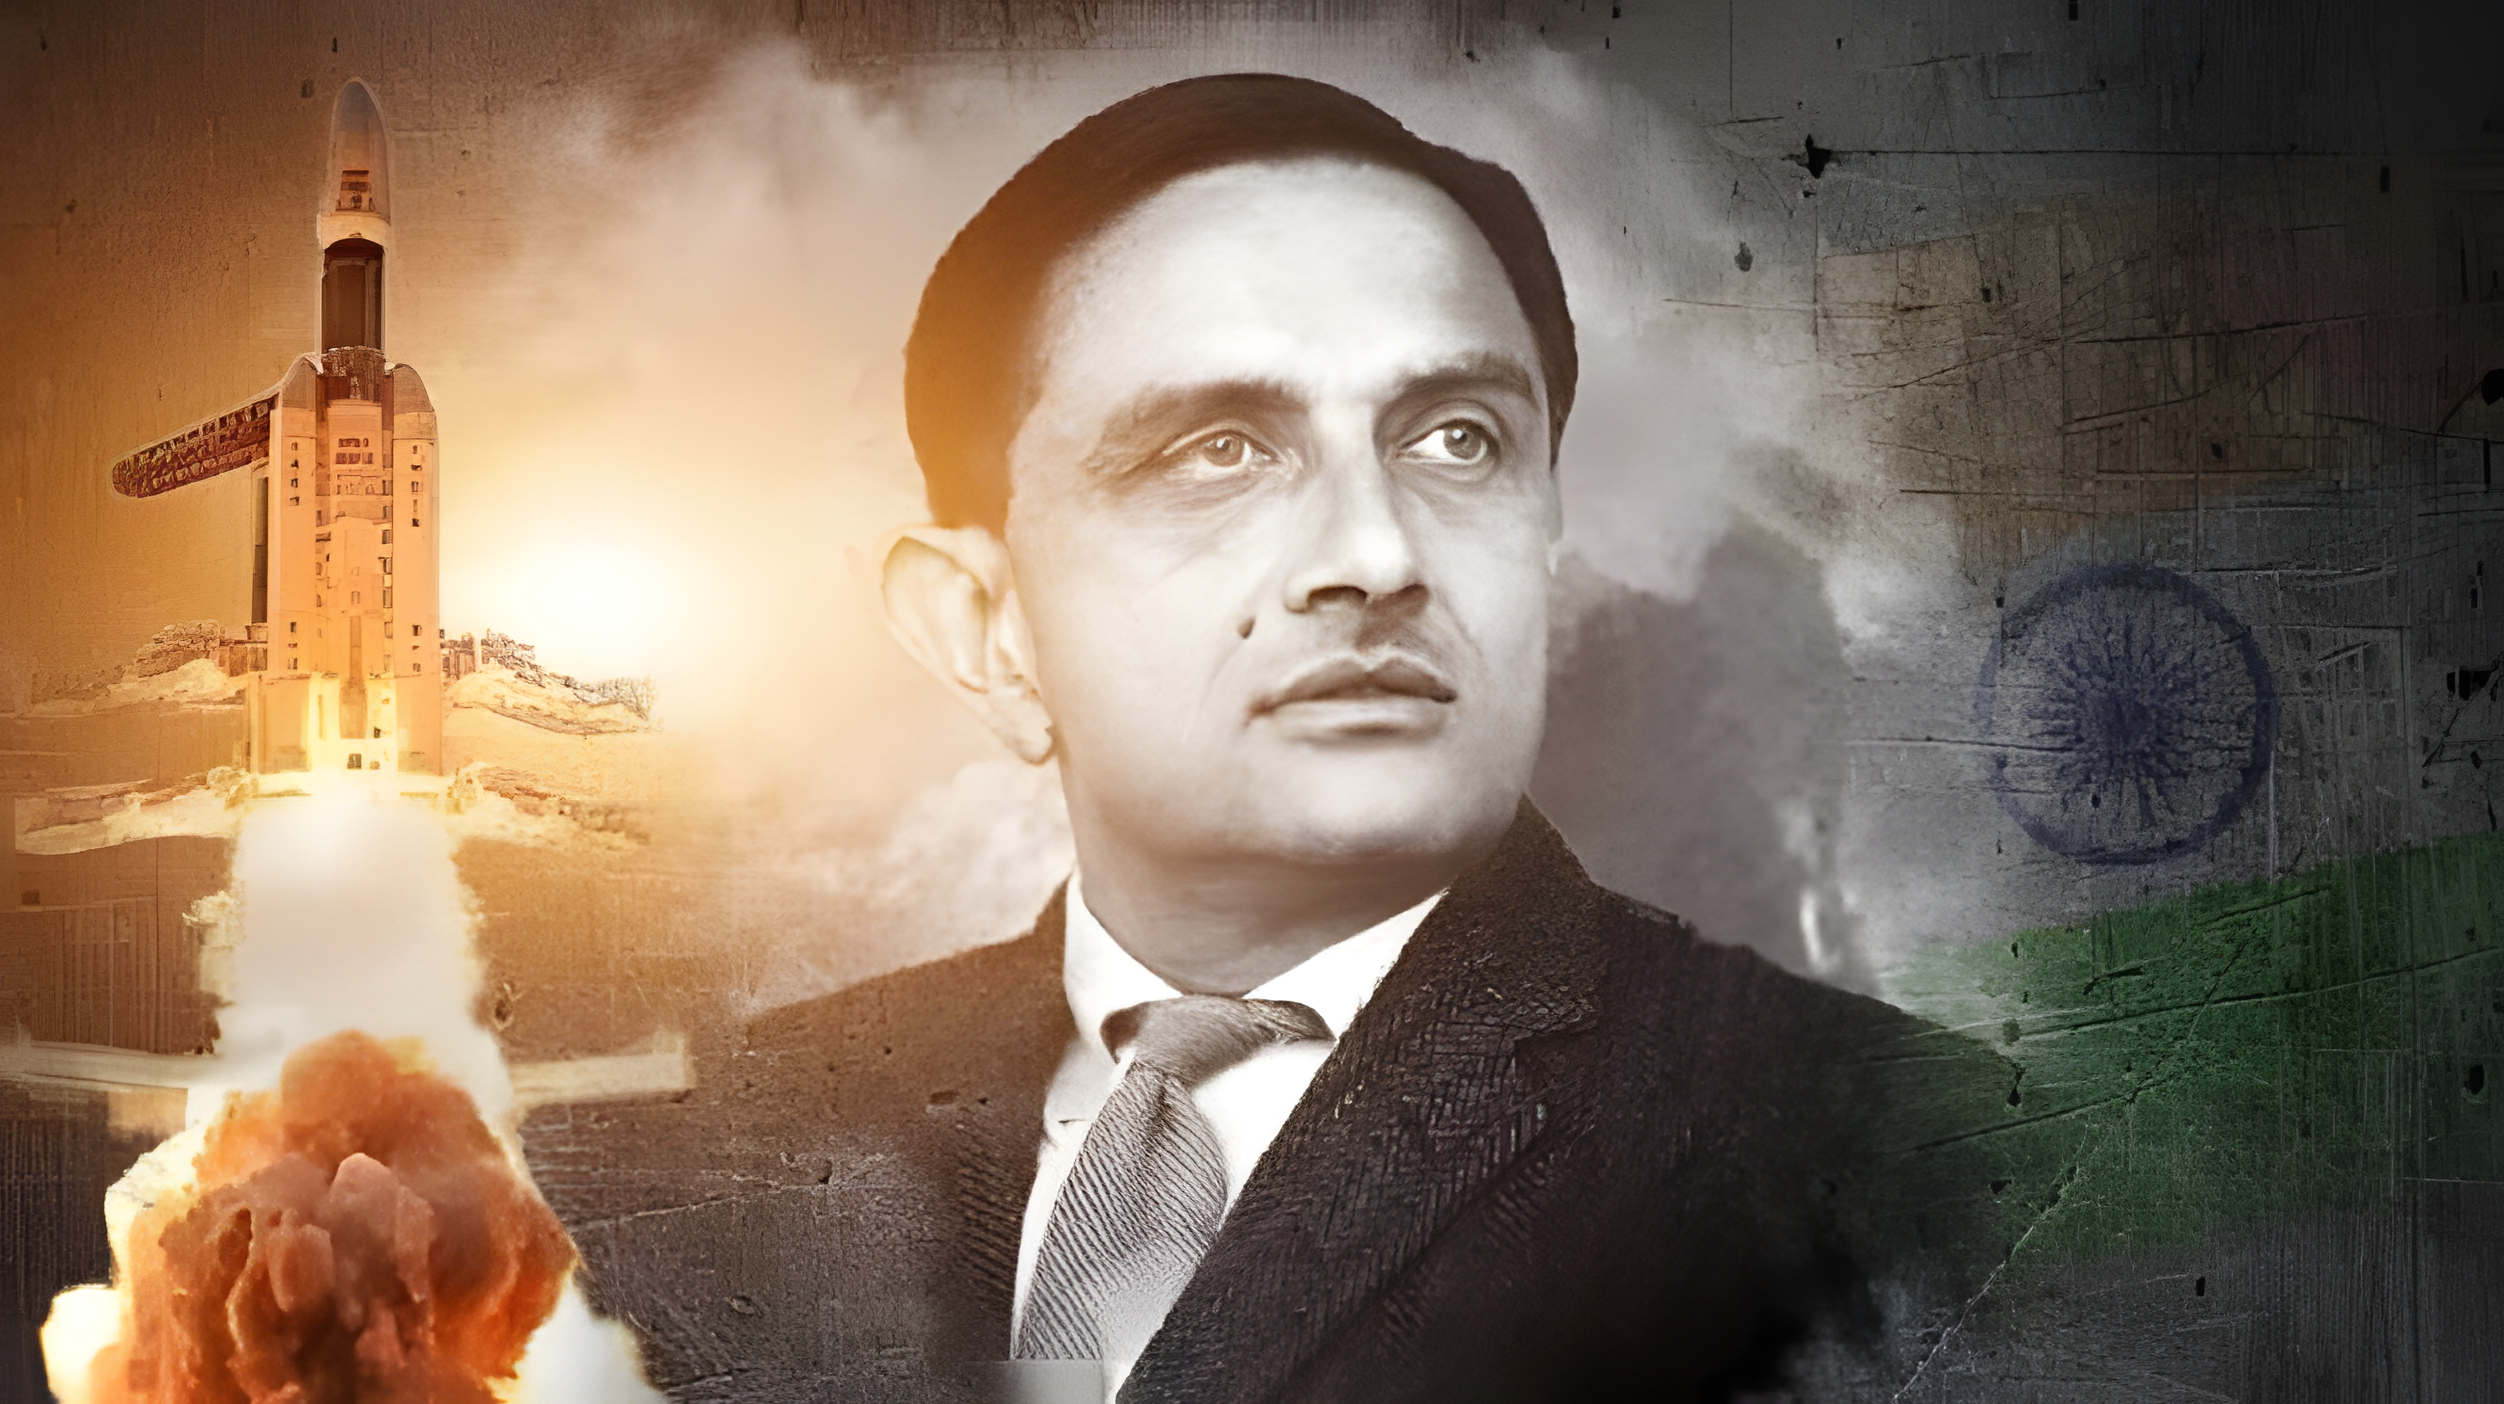
\includegraphics[width=0.85\columnwidth]{assets/images/VAS.png}
    \captionof{figure}{Dr. Vikram Ambalal Sarabhai (12 August 1919 – 30 December 1971) an extraordinary Indian physicist,
      astronomer, and industrialist. He is widely revered as the "Father of the Indian Space Program." He was the
    visionary founder of the Indian Space Research Organisation (ISRO)}
\end{minipage}
  \end{center}

  ISRO does far more than exploration. The satellites carry television signals, mobile networks, monitor
  monsoon pattern, issue warnings during natural calamities., The data are fed into agricultural planning
  and forest management systems across the country. Remote sensing has heavily transformed India’s
  management in water, land, and urban growth. The flagship missions Chandrayaan, Mangalyaan,
  Aditya-L1 grabbed spot in global headlines. NavIC quietly became one of the strategic asset providing
  intel and data to Indian military. Gaganyaan, the upcoming project promises to place India among the very few nations capable of crewed spaceflight. We as Indian students grown up watching ISRO
  succeed, and many are now building the future in AI, robotics, aerospace and more with ISRO.

  {\centering
  \vspace{-0.3em}
  \begin{minipage}{0.98\columnwidth}
  \centering
    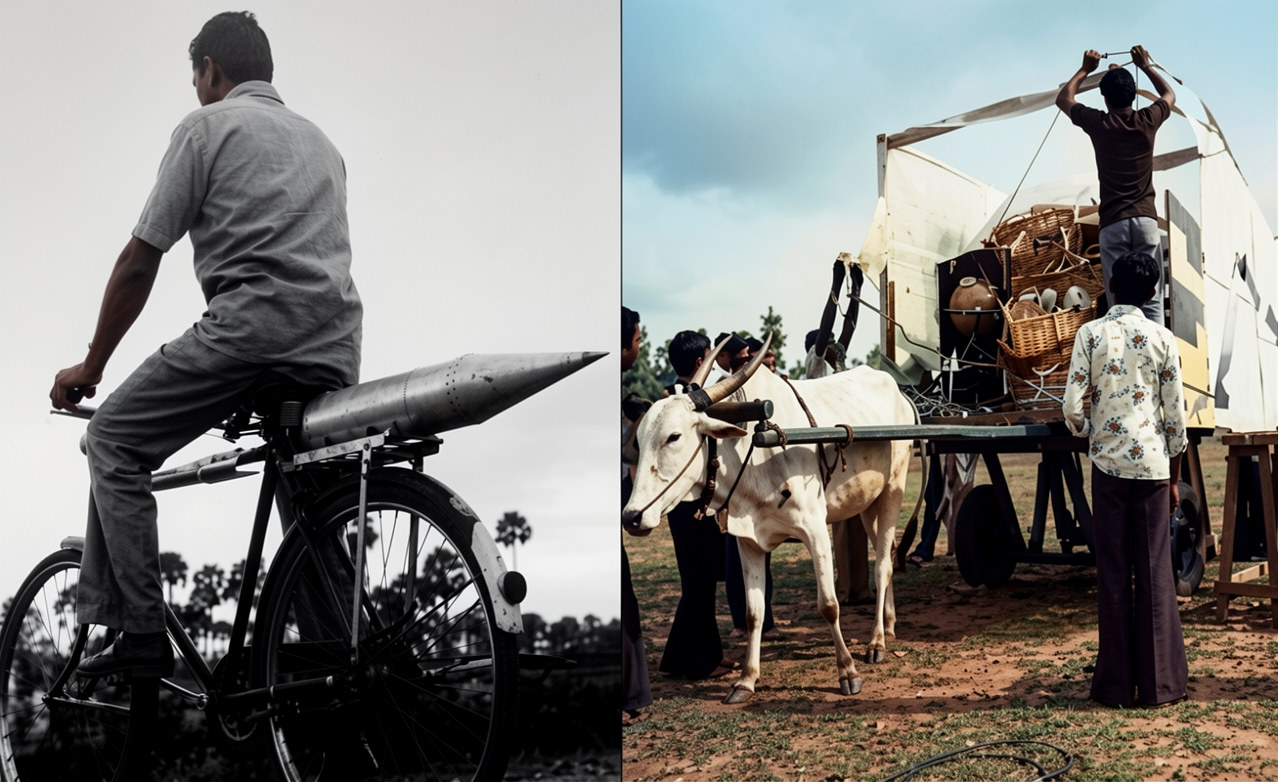
\includegraphics[width=0.85\columnwidth]{assets/images/CRS.jpg}
    \captionof{figure}{The iconic historical photograph shows an Indian space scientist carrying a rocket nose cone on the back of a
      bicycle features scientist CR Satya[11], while a young Dr APJ Abdul Kalam[12] was an integral part of the same
    early rocket launch team.}
  \end{minipage}\par}
  \vspace{-0.4em}

  \subsection*{\centering\uppercase{EVOLUTION AND GROWTH OF ISRO}}
  ISRO began operations on 15 August 1969 i.e. on the eve of India's 22nd Independence Day. Dr.
  Vikram Sarabhai's (one of the founding members) had a straightforward vision i.e. space technology
  should contribute to national development. India recognised early that space research could directly
  address the country's social and economic problems. To solve this the organisation contributed
  tirelessly on research, innovation, and building capability from within despite having limited funding
  or resources during initial years.
  \par\noindent
  The first significant milestone was achieved in 1975 with launch of Aryabhata[13], India's first
  satellite. It wasn't sophisticated according to global standards, but it laid the foundation that could be
  built upon. From there, ISRO developed successive launch vehicle families: the SLV, then the
  PSLV[14], then the GSLV[15], each generation more advanced than the last.

  \begin{center}
\vspace{-0.5em}
\begin{minipage}{0.98\columnwidth}
\centering
    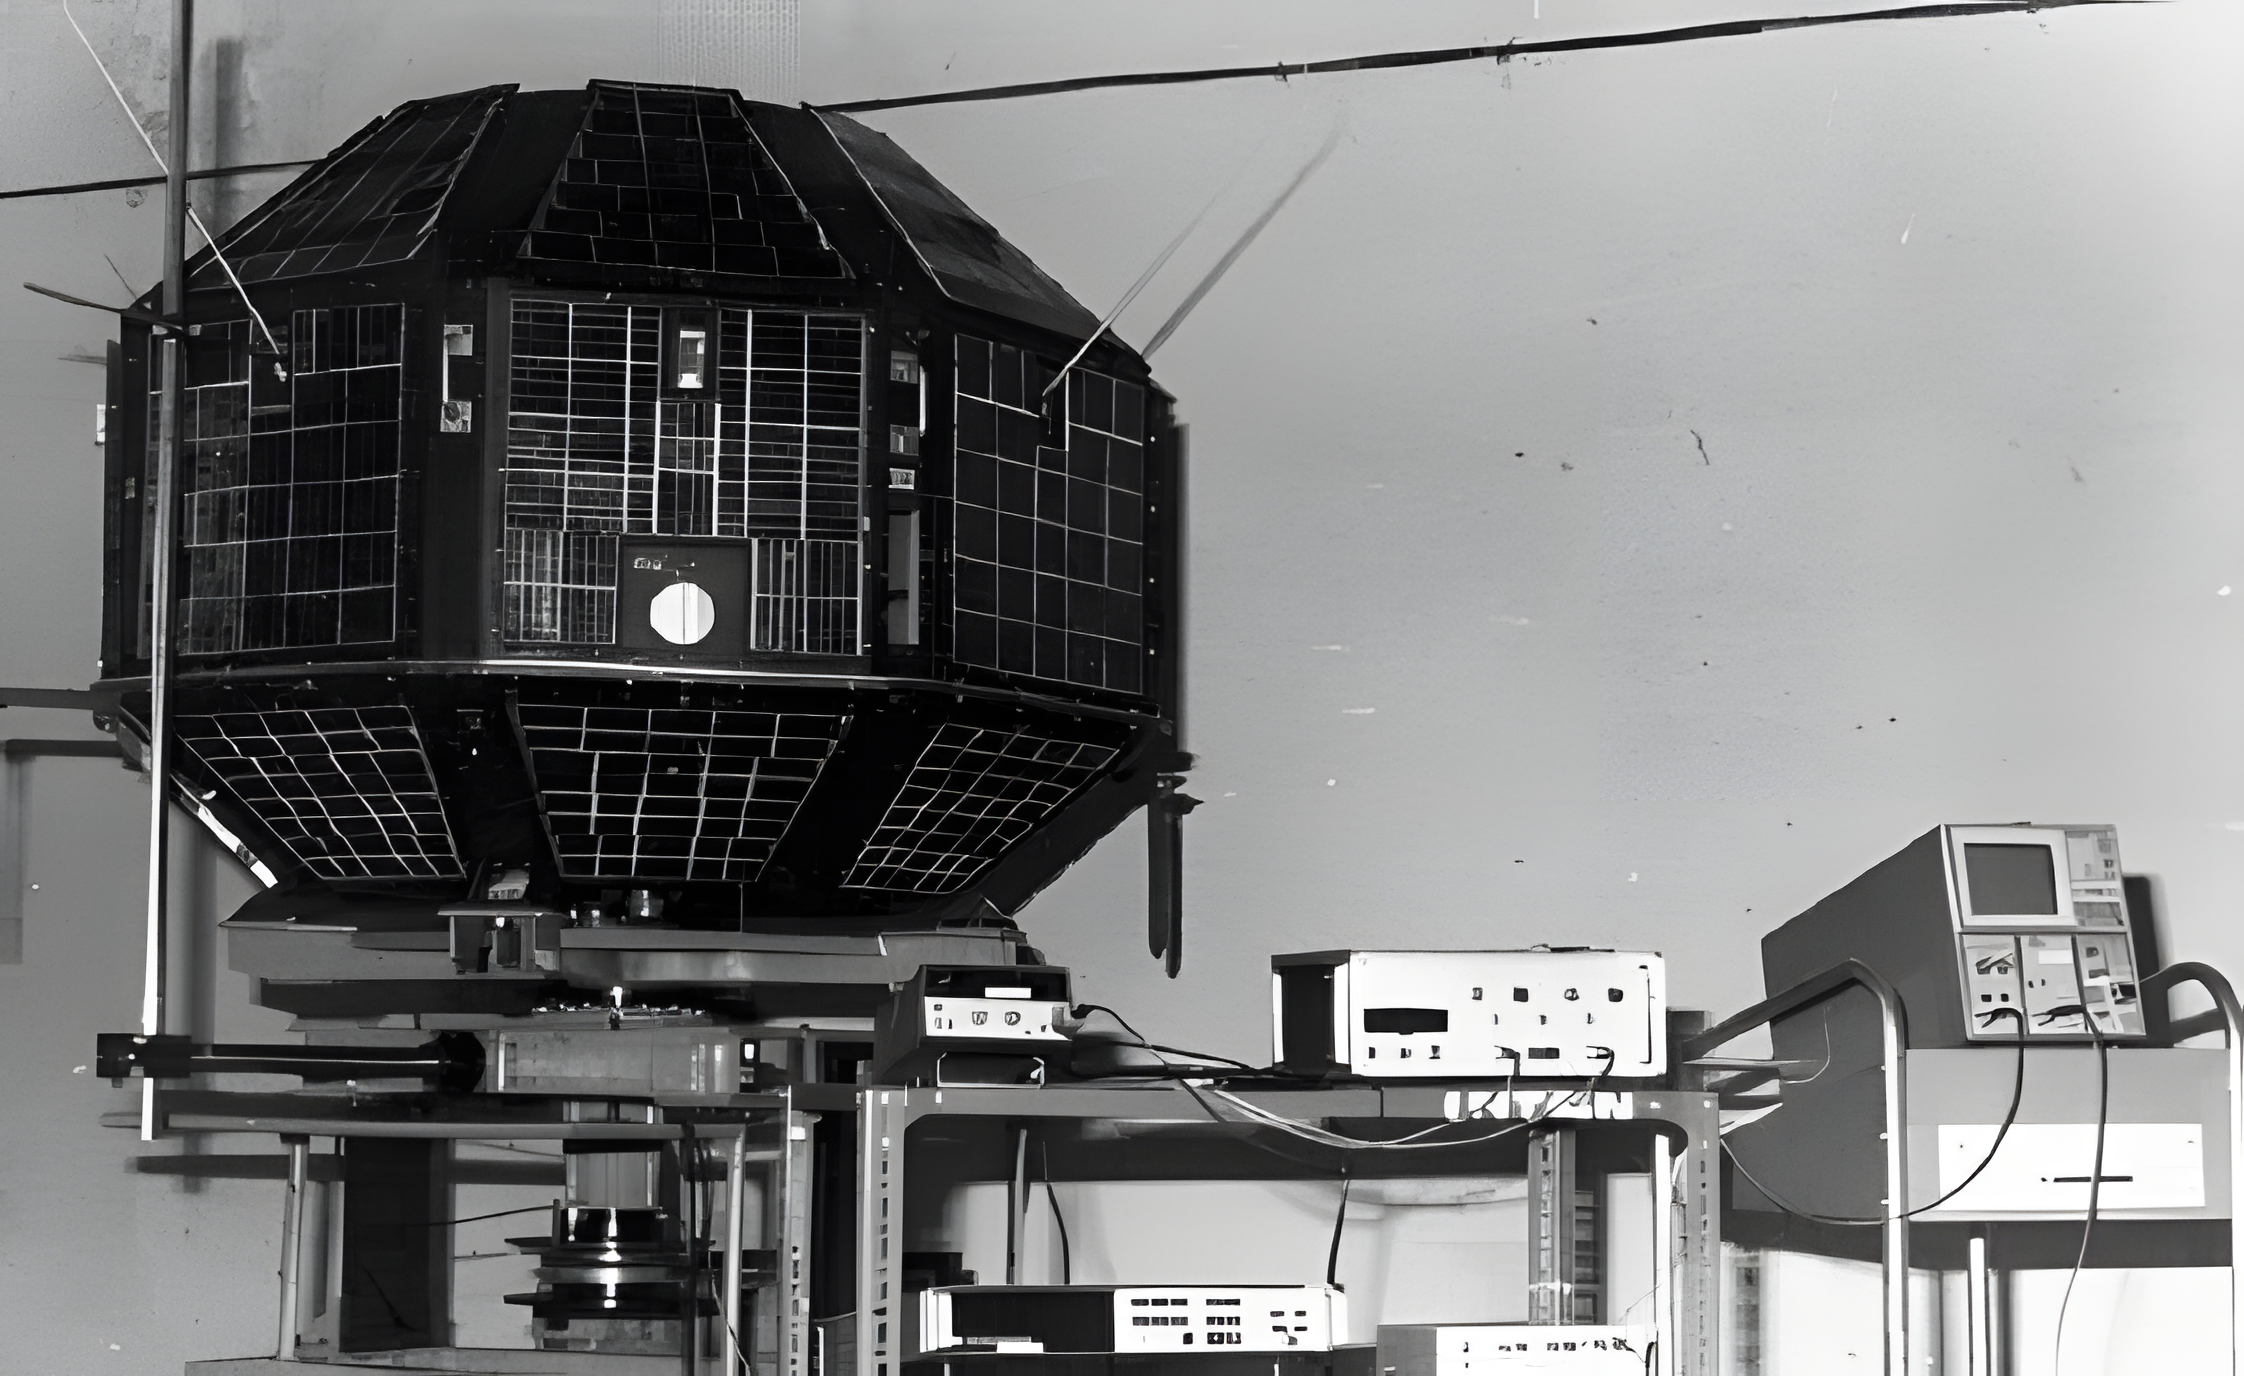
\includegraphics[width=0.7\columnwidth]{assets/images/Aryabhatta.png}
    \captionof{figure}{Aryabhata was India's first satellite, launched on April 19, 1975, from the Kapustin Yar rocket launch site in the Astrakhan
      Oblast, Soviet Union (present-day Russia), utilizing a Kosmos-3M launch vehicle. The 360-kilogram satellite was designed and
    fabricated entirely by the Indian Space Research Organisation (ISRO)}
\end{minipage}
  \end{center}

  The ability to launch independently meant India no longer needed to negotiate with foreign agencies
  every time when it needed to launch a satellite. Out of all in SLV series the PSLV became the standout
  due to its reliable, accurate, and cost-effective approach. As a result it earned international recognition
  and attracted commercial launches from foreign clients such as SpaceX, NASA. This proves the
  reliability and success of this organisation. ISRO's trajectory is worth noting: technological
  advancement doesn't require unlimited budgets or inherited infrastructure. All it takes is clear
  priorities, patience, and scientists willing to solve real life problems without shortcuts. India built all
  three from itself and now the results speak for themselves.

  \subsection*{\centering\uppercase{SATELLITE COMMUNICATION AND REMOTE SENSING}}
  One of ISRO's most significant contribution to society is satellite communication. The communication
  satellite carries broadcast signals from radio’s and televisions, telephone services, and internet
  connectivity across the country where uniform infrastructure is impossible due to uneven geography.
  Today Rural districts are now increasingly connected with satellite signals rather than roads and
  railways.
  \par\noindent
  Remote sensing is the most important work, which is rarely talked about. It plays a important role in
  monitoring crop health, track forest cover, measure water reservoir levels. The data are then mapped
  into decisions which affects millions of Indians. Farmers use the data received from satellite on
  weather patterns soil conditions to maintain proper crop yield. Fishermen off India's coastline get real
  time guidance on safe fishing zones, natural calamities like cyclone which is genuinely a life-saving
  information

  \begin{center}
\vspace{-1em}
\begin{minipage}{0.98\columnwidth}
\centering
    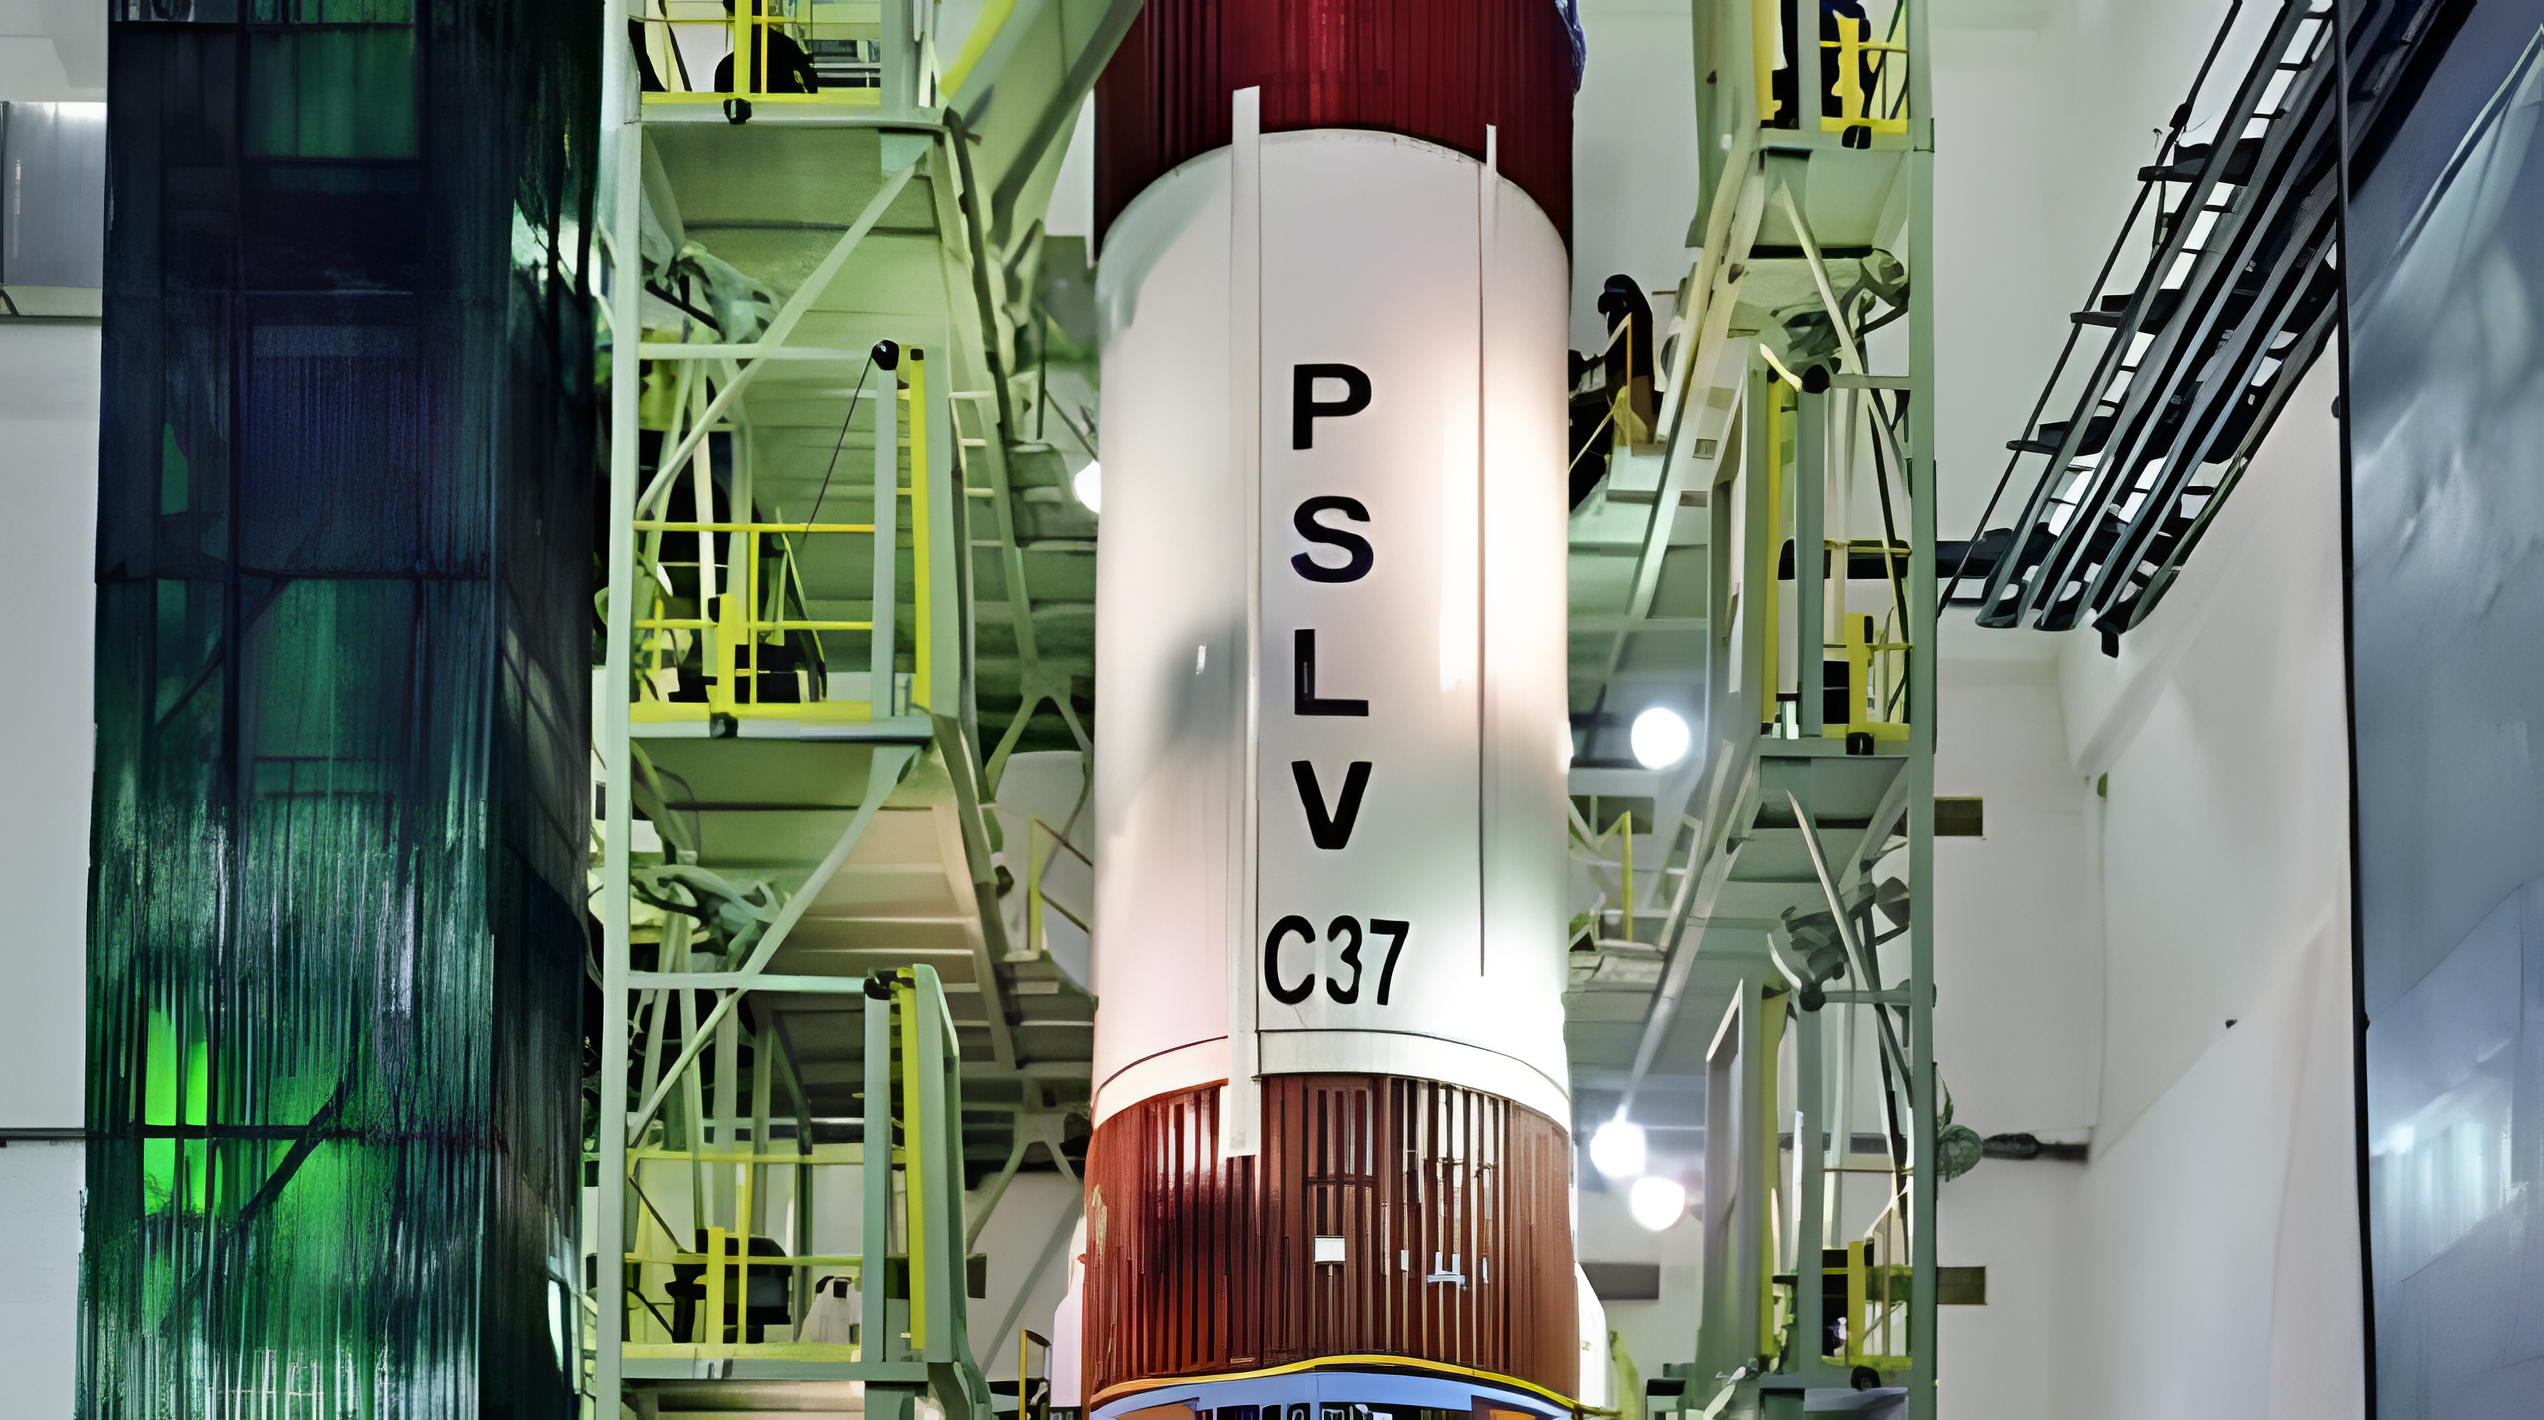
\includegraphics[width=0.85\columnwidth]{assets/images/PSLV.png}
    \vspace{-0.3em}
    \captionof{figure}{PSLV-C37[16] was an historic mission launched by the Indian Space Research Organisation (ISRO) on February 15,
      2017. It successfully deployed a record-breaking 104 satellites in a single rocket flight, which set a global record for the most
    satellites launched in one mission at the time}
\end{minipage}
  \end{center}
\vspace{-0.9em}

  Government agencies previously used to depend on slow and expensive ground surveys. Now days the
  data obtained from satellite are used for land mapping, environmental protection, and infrastructure
  planning work. It not only reduces timeline dramatically, but also provide a improved result. Altogether
  these applications illustrate how ISRO became important for every Indian in day-to-day life. Launch
  records and planetary missions attract attention, but deeper contribution lies in agriculture, natural
  disaster response, fisheries which rarely makes to headlines.

  \subsection*{\centering\uppercase{WEATHER FORECASTING AND DISASTER MANAGEMENT}}
  India is highly vulnerable to wise range of disaster and natural calamities. Cyclone destroy the
  coastlines, floods swallow river plains, droughts stretch across the interior. ISRO's satellite systems
  provide accurate, timely information which is required to prevent catastrophe. Weather data from
  ISRO's satellite is fed directly to early warning systems which give coastal authorities, coast guards
  enough lead time to evacuate people before cyclones make landfall. This capability alone has
  measurably reduced casualties over the past two decades. Satellite imaging-based flood monitoring
  helped disaster management teams to respond affected areas quickly rather than waiting for ground
  reports.

  \begin{center}
\vspace{-0.5em}
\begin{minipage}{0.98\columnwidth}
\centering
    \vspace{-0.2em}
    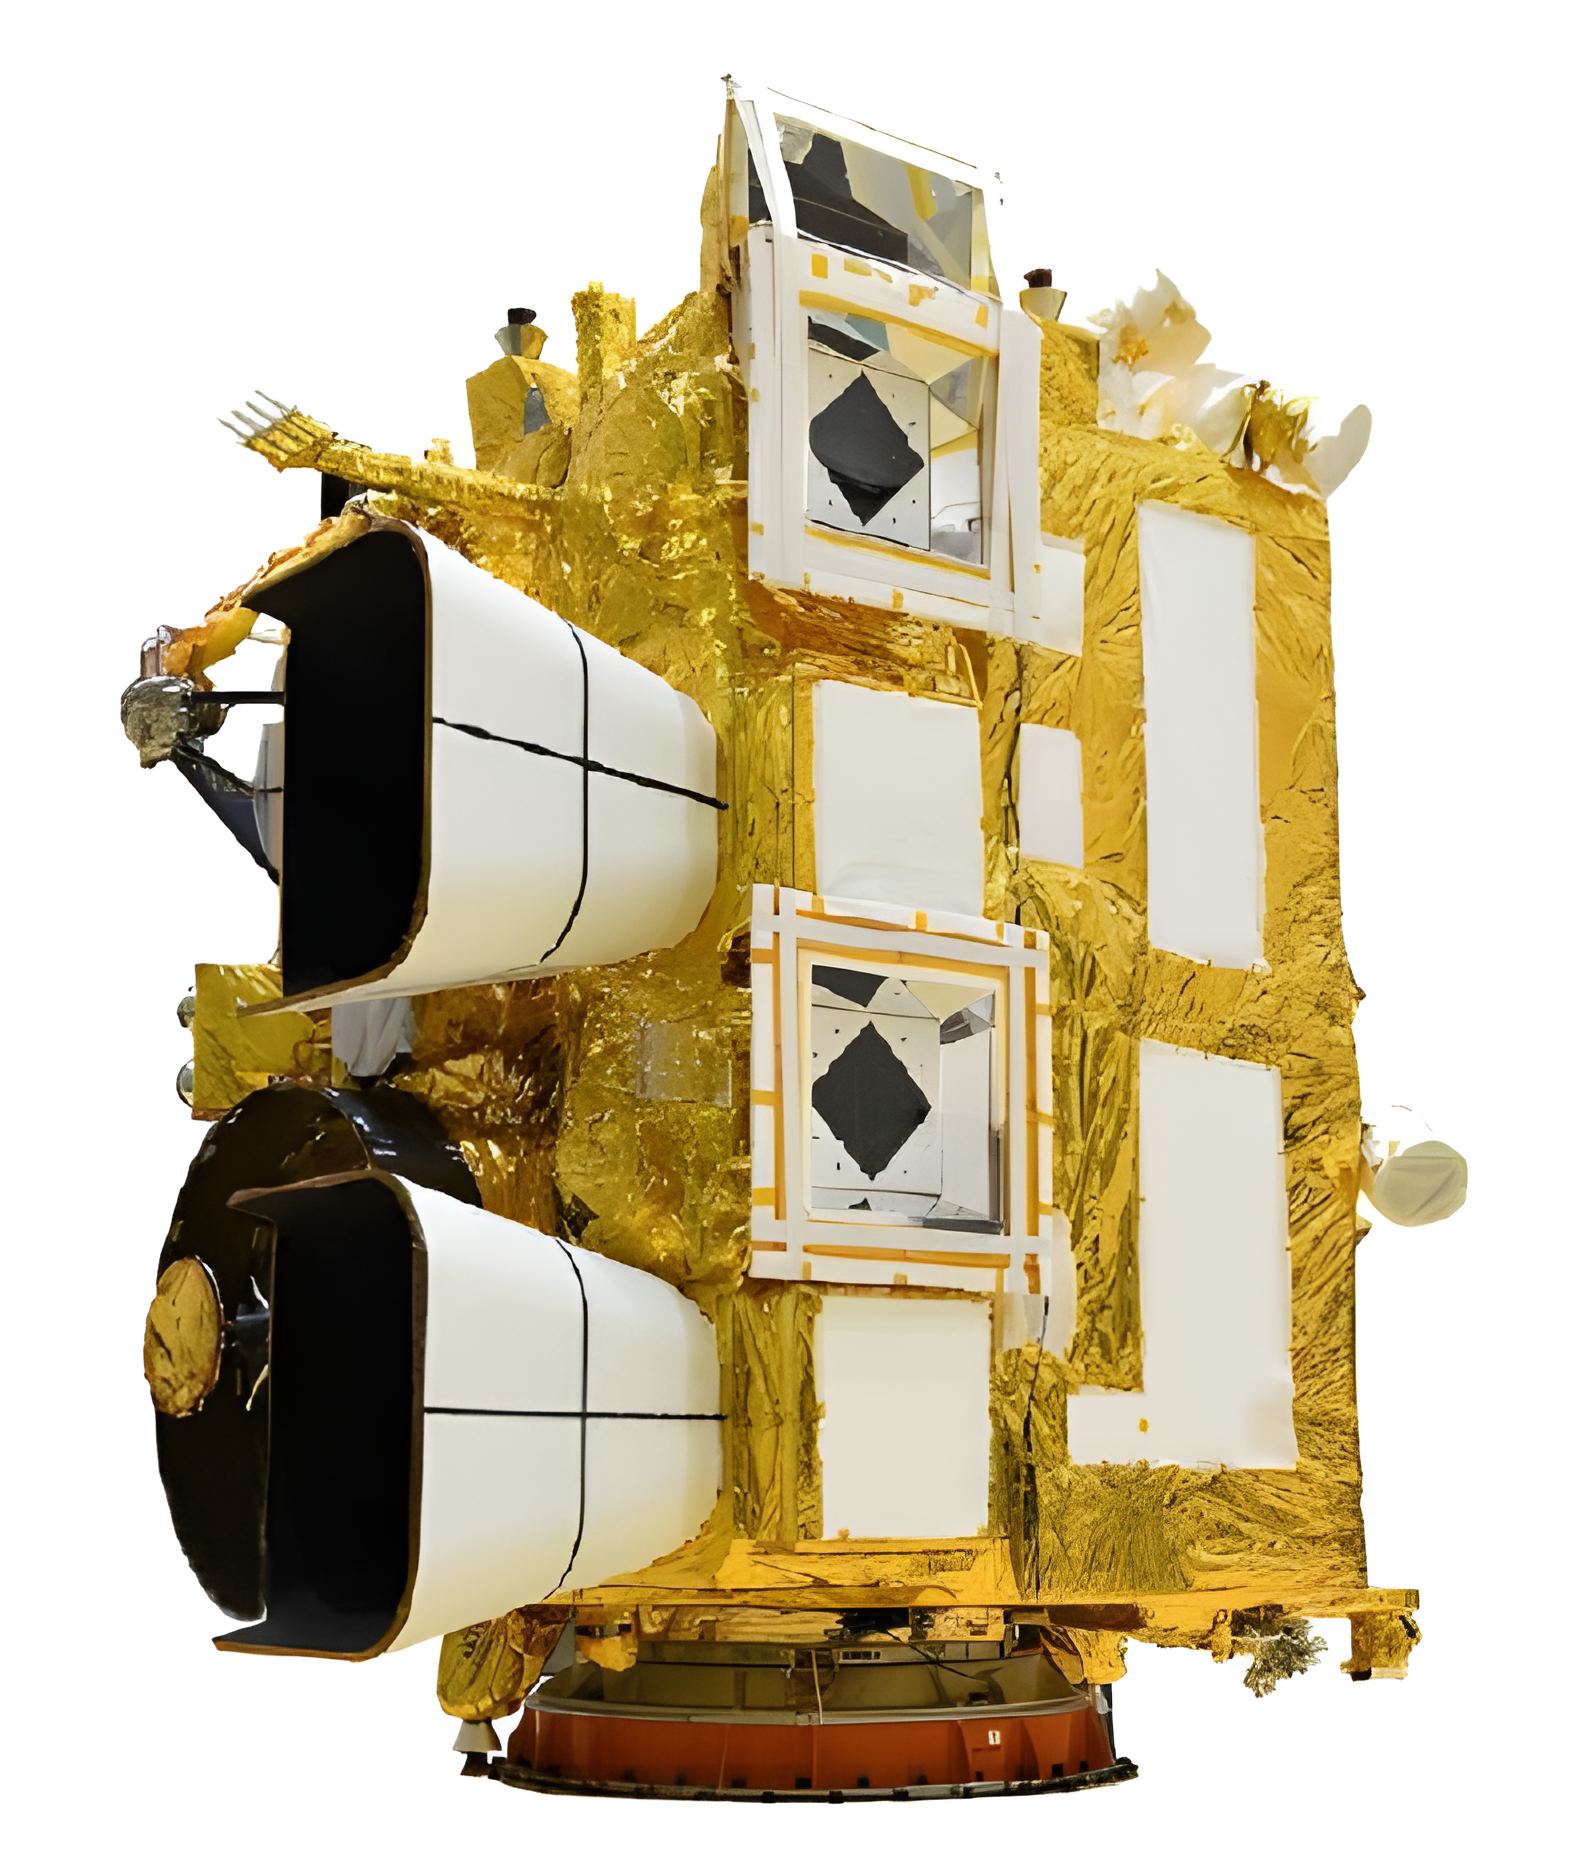
\includegraphics[width=0.75\columnwidth]{assets/images/INSAT.png}
    \captionof{figure}{INSAT-3DS[17] is an advanced meteorological and oceanic observation satellite launched by ISRO on February 17,
      2024. Fully funded by the Ministry of Earth Sciences (MoES), it serves as a follow-up mission to INSAT-3DR[18] and INSAT-
    3D[19]. The satellite enhances India's weather forecasting, climate monitoring, and disaster warning capabilities}
    \vspace{-0.4em}
\end{minipage}
  \end{center}
  \vspace{-0.3em}
  The most significant part isn’t the technology it’s the impact. Space infrastructure is built and operated
  thousands of kilometres above the earth surface. This infrastructure is actively protecting lives in fishing
  villages, river deltas, and hill and mountain region across India. This is how space research contributes
  to human welfare and is more important than any planetary mission.

  \subsection*{\centering\uppercase{NAVIGATION SYSTEMS AND NATIONAL SECURITY}}
  Another technological advancement for ISRO is the development of Navigation with Indian
  Constellation (NavIC). NavIC is India's regional navigation system just like GPS. It provides accurate
  positioning and timing services. The system reduces India's dependence on foreign navigation systems
  like GPS and strengthens technological self-reliance.
  \par\noindent
  NavIC consists of set of seven satellites which includes IRNSS-1A, IRNSS-1B, IRNSS-1C, IRNSS-
  1D, IRNSS-1E, IRNSS-1F, and IRNSS-1G. The system covers India and a region which extends up to
  1500 km beyond the border. NavIC has been implemented in transportation, maritime navigation,
  disaster management and defence purpose due to its precise and reliable data. With advancement in AI
  and drone tech accurate navigation systems are essential for national security and defence purposes.
  During emergencies and strategic operations, NavIC ensures reliable communication and positioning
  services. It played an crucial role in Operation Sindoor and India Pak War.

  \begin{center}
\vspace{-0.5em}
\begin{minipage}{0.98\columnwidth}
\centering
    \vspace{-0.4em}
    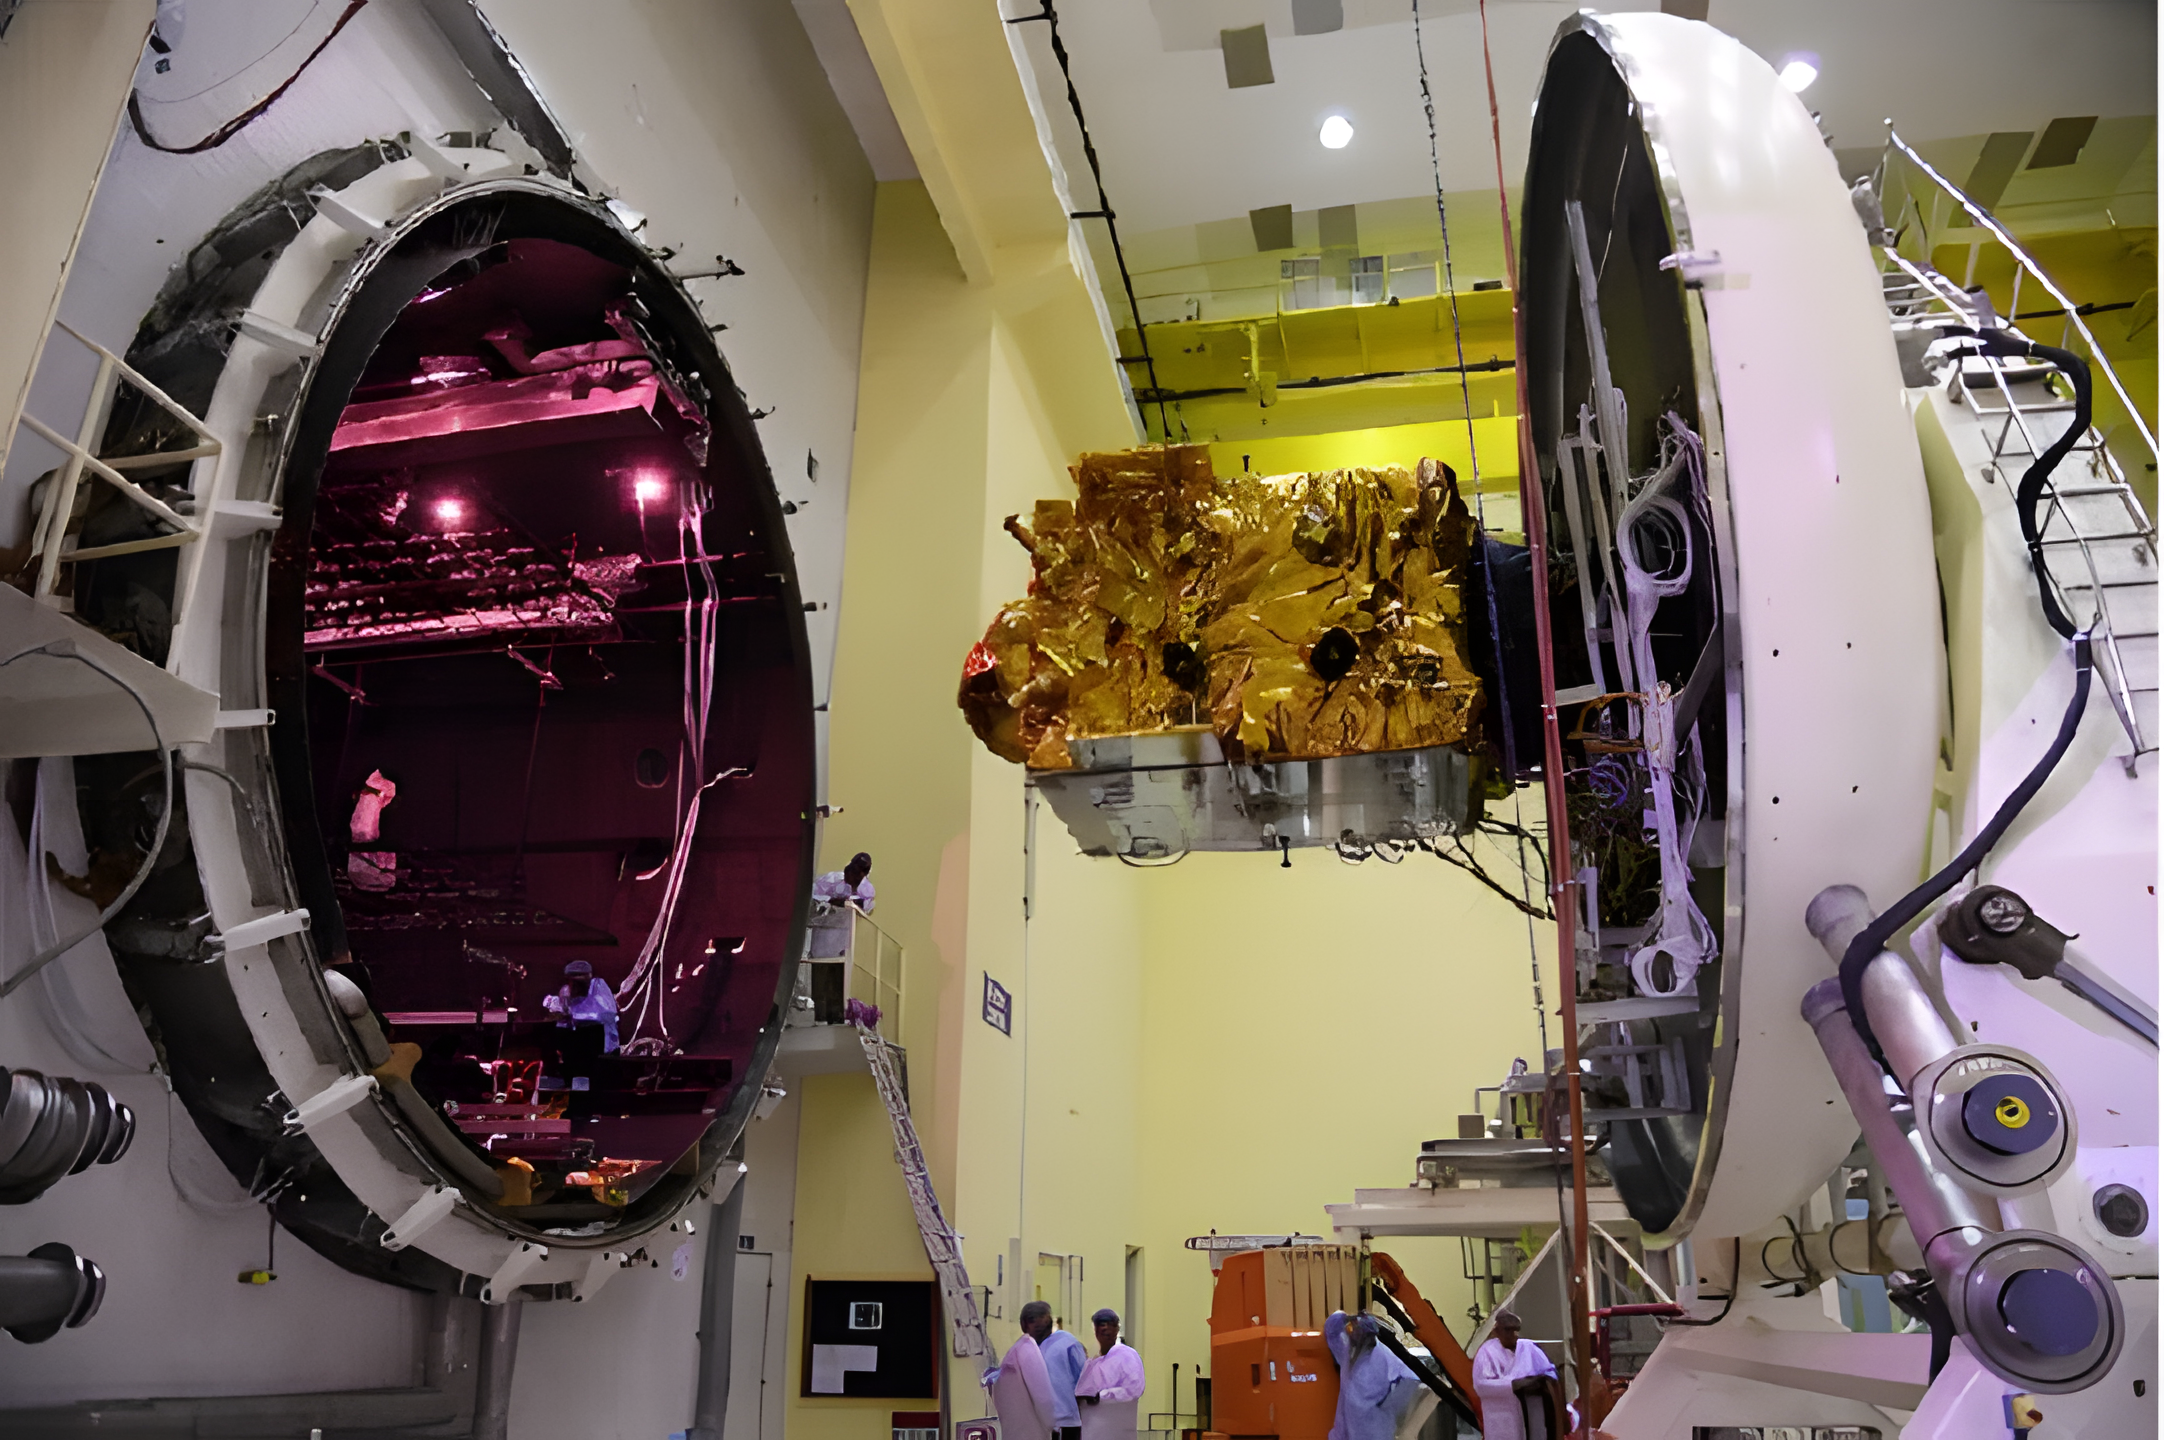
\includegraphics[width=0.75\columnwidth]{assets/images/NavIC.png}
    \captionof{figure}{NavIC (Navigation with Indian Constellation) is India's indigenous regional satellite navigation system developed by
      ISRO. It provides highly accurate real-time positioning, velocity, and timing services across the Indian landmass and up
    to 1,500 km beyond its borders, functioning as a localized, independent alternative to GPS.}
    \vspace{-0.6em}
\end{minipage}
  \end{center}
  \vspace{-0.5em}
  ISRO has also contributed to national security through surveillance satellites and communication
  systems. These technologies support border monitoring, defense operations, and intelligence gathering.
  They strengthen India's security infrastructure.

  \subsection*{\centering\uppercase{MAJOR SPACE MISSIONS}}
  ISRO's mission record proves the organisation’s ability and capability to achieve successful results
  despite limited resources and funding. Chandrayaan-1, India’s first lunar mission launched in 2008
  found evidence of water molecules on the lunar surface. The discovery urprised the international
  scientific and scholar community and questioned traditional thinking about the Moon's history.
  Chandrayaan-2[20] successor of that program failed in the terminal phase when landing during landing
  on south pole. Chandrayaan-3[21] achieved a soft landing near the Moon's south pole, making India
  the fourth country to land on moon. The south is important in scientist community because it is where
  the trapped ice is expected

  \begin{center}
\vspace{-0.5em}
\begin{minipage}{0.98\columnwidth}
\centering
    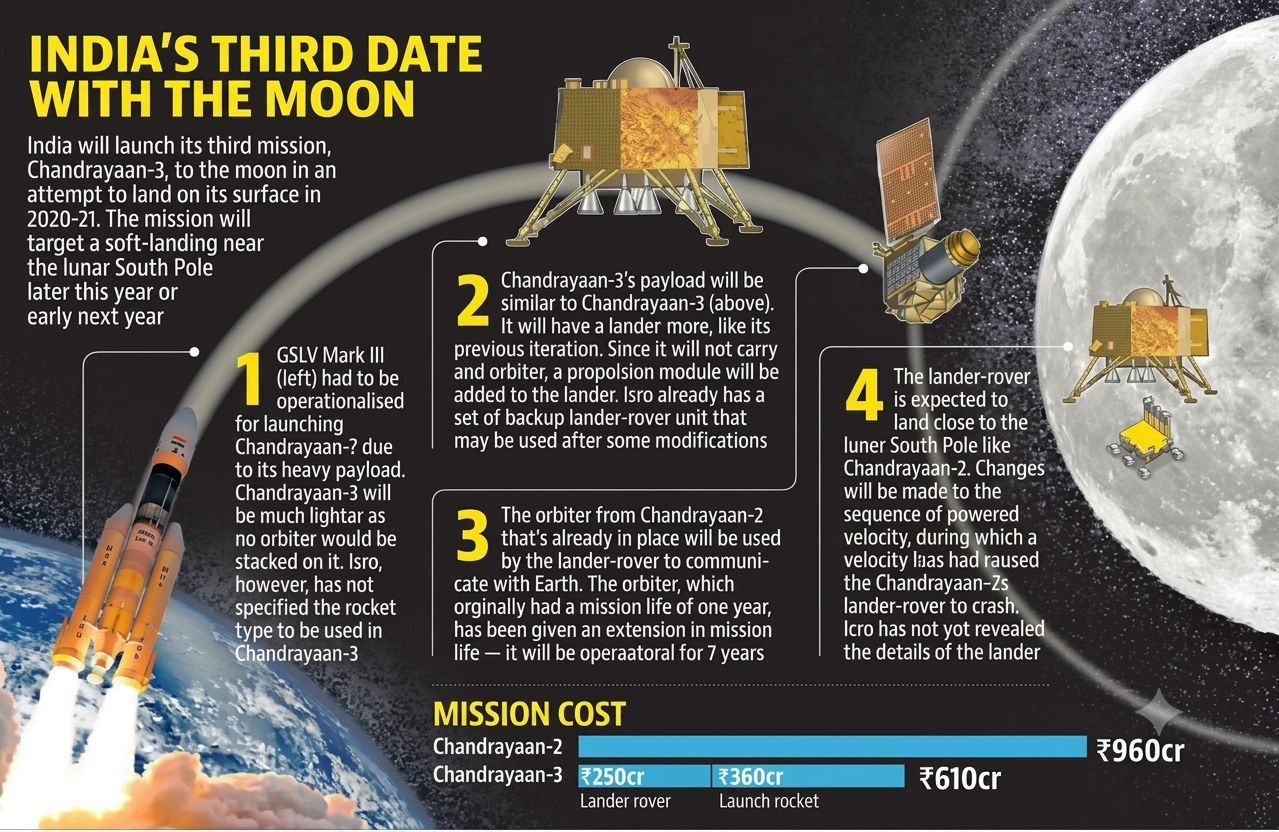
\includegraphics[width=0.8\columnwidth]{assets/images/ITD.png}
    \captionof{figure}{India's Chandrayaan program is a series of lunar exploration missions developed by the Indian Space Research Organisation
      (ISRO). It began in 2008 with Chandrayaan-1, an orbiter mission that famously discovered water on the Moon. This was followed
      by Chandrayaan-2 in 2019, which successfully deployed an orbiter but suffered a lander crash. Chandrayaan-3 successfully
    achieved a historic soft landing at the lunar south pole in 2023.}
\end{minipage}
  \end{center}

  Mangalyaan arrived at Mars in 2014 on India's first attempt at a budget almost half of Interstellar
  movie. The engineering was elegant, the budget was tight, and it worked.

  \begin{center}
\vspace{-0.5em}
\begin{minipage}{0.98\columnwidth}
\centering
    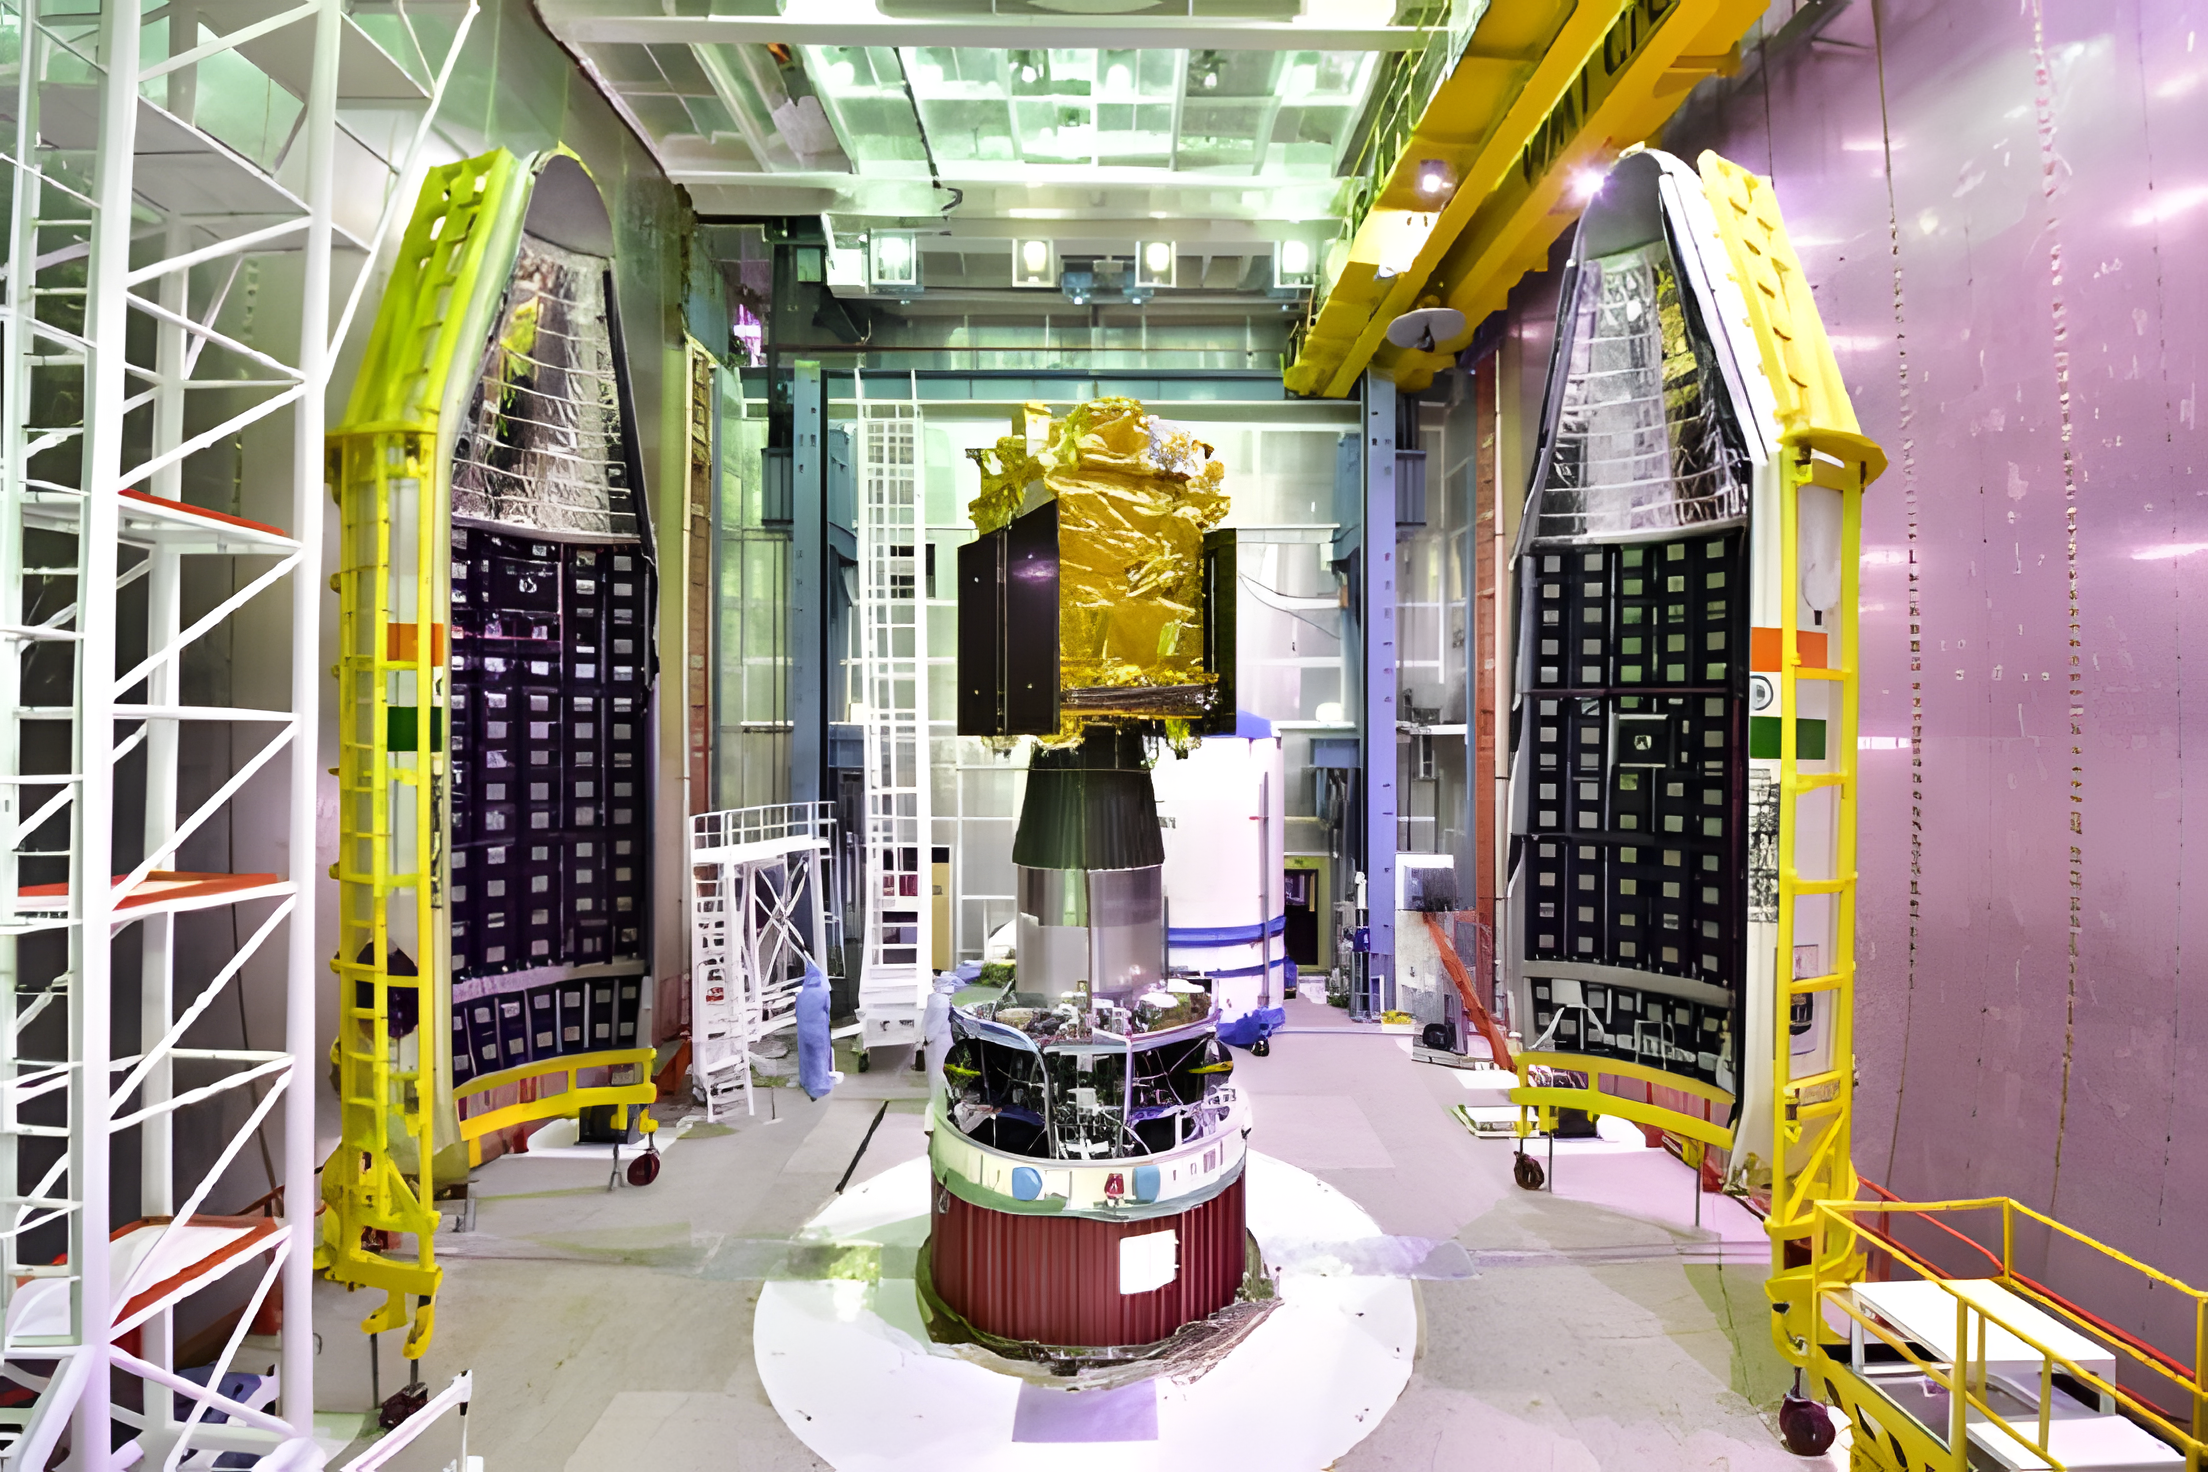
\includegraphics[width=0.65\columnwidth]{assets/images/MOM.png}
    \captionof{figure}{Mangalyaan, officially known as the Mars Orbiter Mission (MOM), is the Indian Space Research Organisation’s (ISRO)
      Mars Orbiter Mission - ISRO maiden interplanetary space probe. Launched on November 5, 2013, it successfully entered Martian
    orbit on September 24, 2014, making India the first nation to achieve this in its first attempt}
\end{minipage}
  \end{center}
\vspace{-0.4em}

  Aditya-L1, now stationed at the Sun-Earth L1 point, is used to study solar activity and space weather.
  It is highly important as all satellite infrastructure are highly vulnerable to solar events. Gaganyaan
  India's first crewed mission is the upcoming project. If it succeeded it would place India would be the
  fourth country in the world to have sent humans to space independently. The bar is extremely high as
  any single fault would cost human lives .ISRO is conducting exhaustive testing to master the
  technology

  \begin{center}
    \begin{minipage}{\columnwidth}
    \centering
    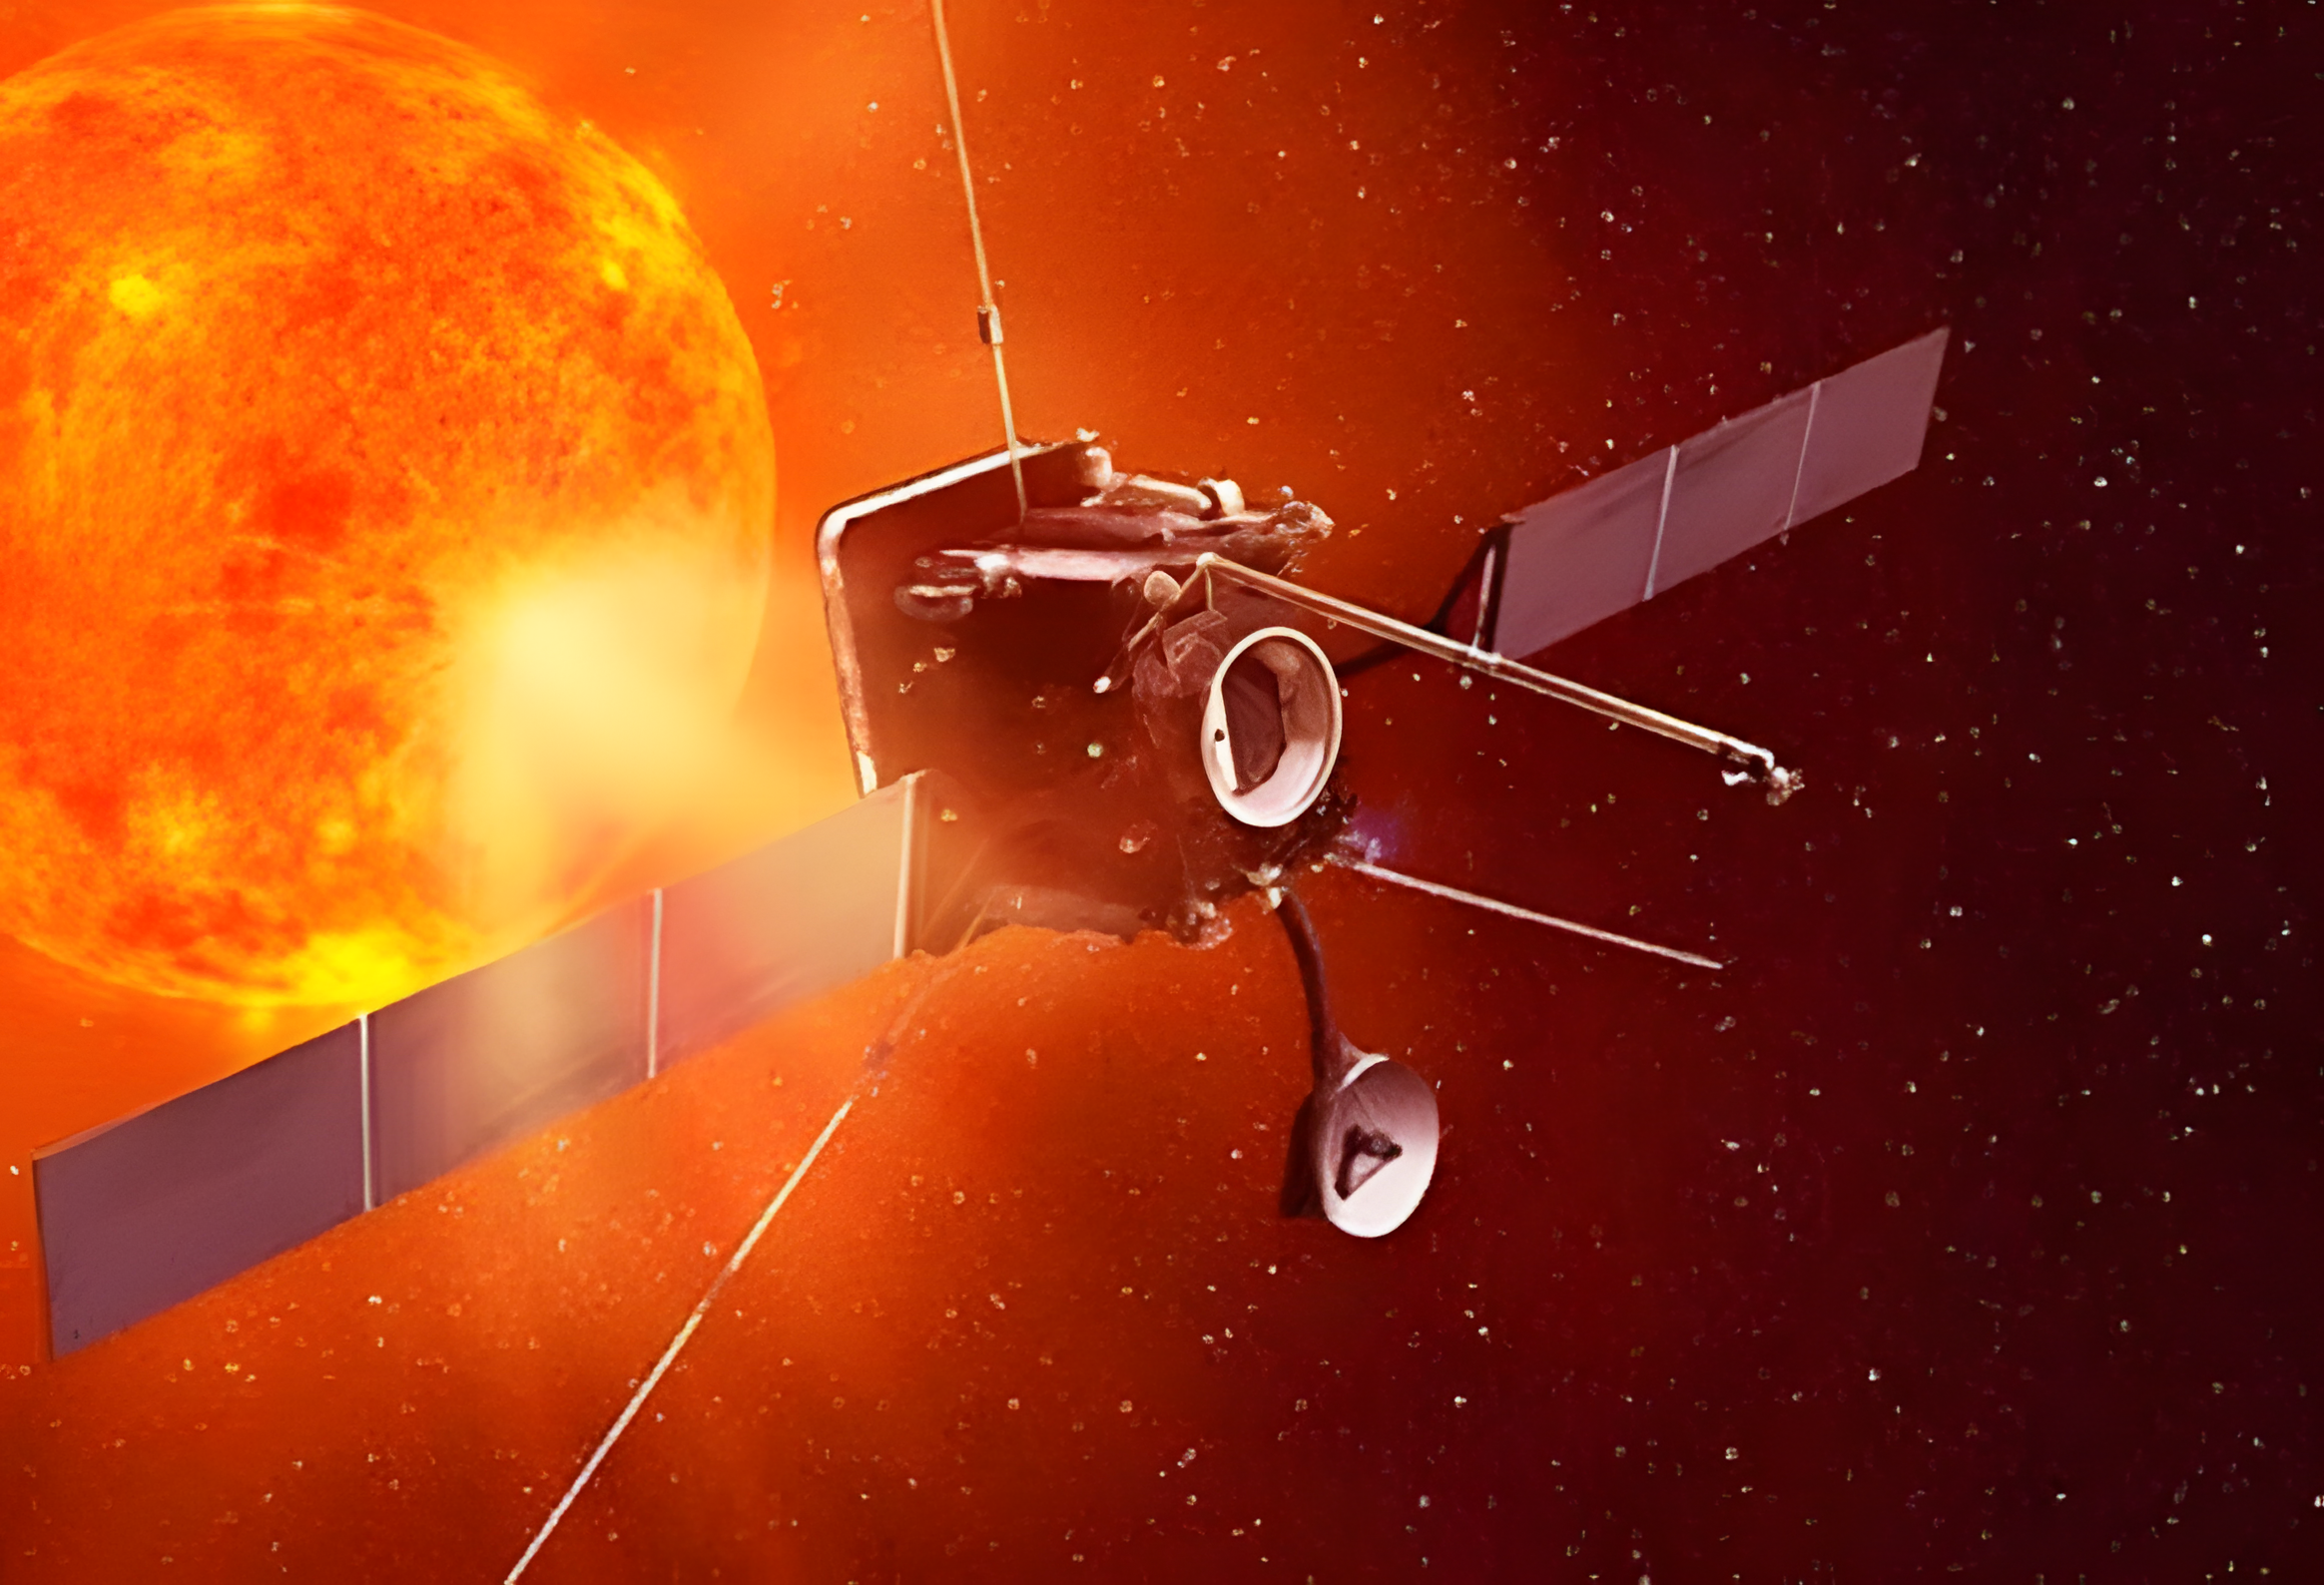
\includegraphics[width=0.85\columnwidth]{assets/images/AL1.png}
    \captionof{figure}{Aditya-L1, India’s first dedicated solar observatory, studies the Sun and space weather from the Sun--Earth L1 point.}
    \end{minipage}
  \end{center}
  \subsection*{\centering ISRO'S CONTRIBUTION TO SCIENCE, EDUCATION, AND INDUSTRY}
  The achievements of the Indian Space Research Organisation (ISRO) have boosted interest and
  curiosity in science and technology among Indians. Watching Mangalyaan reaching Martian orbit and
  Chandrayaan soft landing on south pole have inspired many Indian students to pursue their future
  studies in science and engineering. As a result, fields such as aerospace engineering, robotics, and
  artificial intelligence, once considered unattainable, and distant are now attracting a large number of
  students every year. ISRO collaborates with universities and research institutions to provide
  internships and training opportunities, providing a platform for students to link academic interests
  with practical real world engineering problems. Private enterprises are also increasingly involved in
  space exploration, contributing so rapidly to satellite technology, launch vehicle development, and
  space research that a single government agency cannot keep up.

  \begin{center}
    \begin{minipage}{\columnwidth}
    \centering
    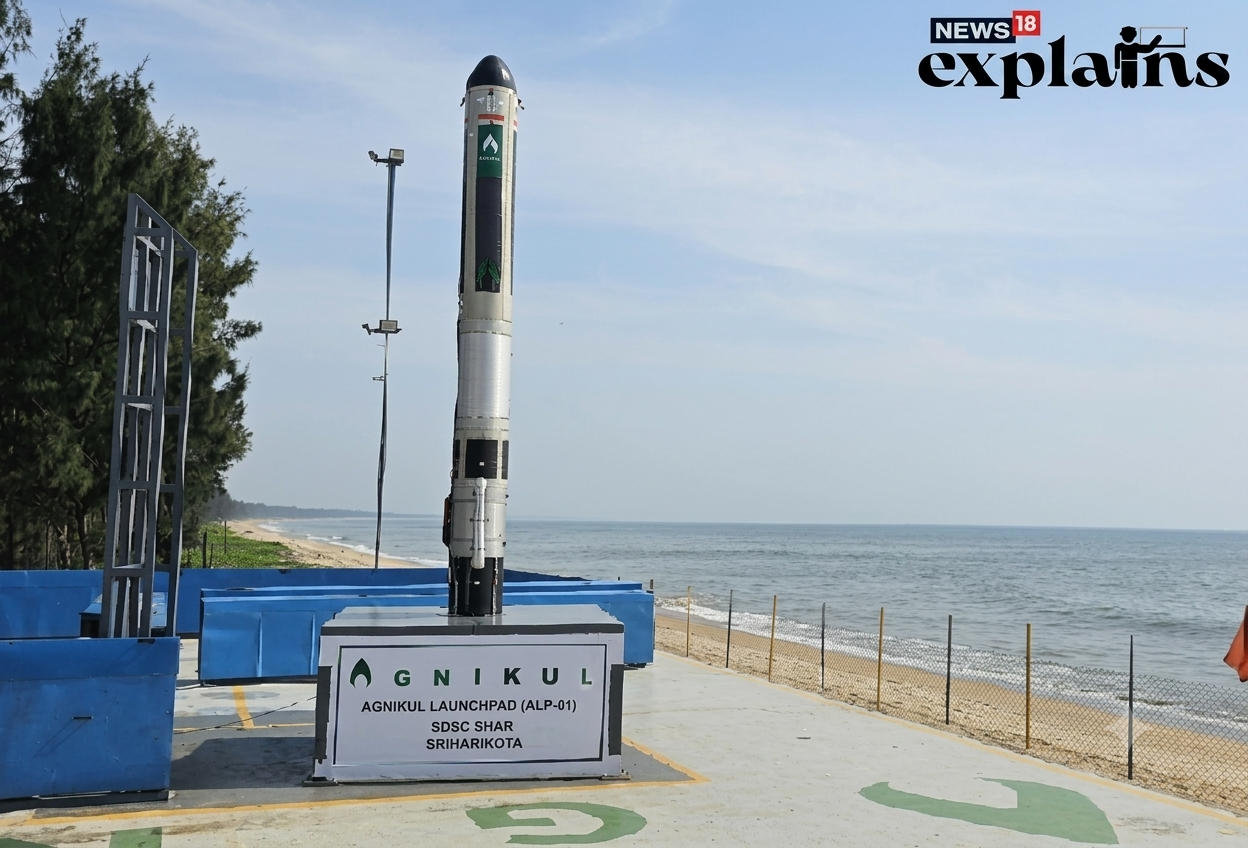
\includegraphics[width=0.85\columnwidth]{assets/images/IITM.png}
    \captionof{figure}{Agnikul Cosmos, an IIT Madras-incubated startup, successfully launched the Agnibaan SOrTeD[22] (Sub-Orbital
      Technology Demonstrator) rocket from Sriharikota, powered by the world's first single-piece 3D-printed semi-cryogenic
    engine. The historic flight validated the startup's in-house 3D printing and software-defined propulsion technologies.}
    \end{minipage}
  \end{center}

  Today the shift from single government agency ISRO to multiple private companies have joined and
  honestly it created more jobs and money . Engineers from startups like Skyroot and Agnikul are us who
  grew up watching from a young age what ISRO has pulled off despite having limited resources or
  funding. As government is pushing towards commercialisation, scientist or engineers who would have
  previously left for NASA or ESA are now staying back in India. But honestly if rockets and satellite are
  kept aside, they have created a sense of culture. It showed what Indian scientists what they are actually
  capable to pull off when system or politics don’t intervene. For a kid who is confused about their career;
  watching ISRO succeed from childhood , makes them feel certain career are actually achievable no
  matter how hard they are. This actually matters more than any policy

  \subsection*{\centering\uppercase{FUTURE PROSPECTS AND CHALLENGES}}
  The future direction is indeed ambitious: reusable rockets, longer-distance space missions, advanced
  satellites—India even once hoped to have its own domestically built space station. Several projects have
  begun development and are no longer just on paper. The challenges are real. The emergence of SpaceX
  has intensified global competition and changed expectations about launch costs. Space debris[23] is no
  longer just a theoretical problem but has become a practical challenge. Satellite infrastructure is facing
  more cybersecurity[24] threats. How to reduce costs while pushing the limits of technology has now
  become a real challenge.

  \par\noindent
  Frankly, the Indian Space Research Organisation (ISRO)'s greatest strength lies in its tangible
  achievements. The successful first Mars landing, the reliable and stable NavIC navigation satellite
  system developed in-house, and its relentless pursuit of innovation—these are no accident; ISRO has
  found viable solutions and persisted in using them in every attempt. The challenges of the future are
  vastly different from those of fifty years ago, but what truly matters remains unchanged. Space is
  becoming central to India's future development. ISRO started almost from scratch. Frankly, there's no
  reason to believe they will stop here.

  \subsection*{\centering\uppercase{CONCLUSION}}
  The story of the Indian Space Research Organisation (ISRO) is an unbelievable tale on how to stretch
  every rupee to its absolute limit, surpassing every person expectation. For over fifty years, they have
  established communication networks, navigation systems, weather forecasting capabilities, and disaster
  warning systems. ISRO have accomplished all this with tight budget and limited resources guided by
  clear and well-defined priorities. Their flagship missions have earned attention worldwide: the
  *Chandrayaan* lunar probe confirmed the presence of water on the Moon; Mangalyaan the *Mars
  Orbiter Mission* successfully reached Mars on its very first attempt; and the *Aditya-L1* probe
  propelled India into the realm of solar physics; fields only a handful of agencies have actually acquired.
  Moreover the underrated efforts such as NavIC system, which reduces reliance on foreign GPS, and
  remote sensing where satellites are used to provide data support for agricultural and environmental
  decision-making likely impact the lives of millions of Indians on a daily basis.
  The future developments of ISRO are equally significant. Gaganyan mission will place India among
  the list of very few countries capable of conducting human spaceflight independently. Deep space
  exploration[25] are beginning to take shape.The growing enterprise of private startups, university
  collaborations, and commercial launches surrounding the Indian Space Research Organisation (ISRO)
  will further accelerate all of this. For India, space technology and national development have never been
  separate goals. ISRO has integrated the two, and this foundation appears solid enough to support
  significant future growth.

  \subsection*{\centering\uppercase{References}}
  \begingroup\justifying
  \Urlmuskip=0mu plus 1mu\relax
  \begin{enumerate}[leftmargin=*,itemsep=0.20em,topsep=0.12em,parsep=0pt]
    \item National Air and Space Museum, “All About Rockets.” [Online]. Available:
      \url{https://airandspace.si.edu/learn/programs/soar-together/rockets-2}.
    \item Indian Space Research Organisation, “Chandrayaan-1.” [Online]. Available:
      \url{https://www.isro.gov.in/Chandrayaan_1.html}.
    \item Indian Space Research Organisation, “Aditya-L1.” [Online]. Available:
      \url{https://www.isro.gov.in/Aditya_L1.html}.
    \item National Aeronautics and Space Administration, “What is a Lagrange Point?” [Online]. Available:
      \url{https://science.nasa.gov/resource/what-is-a-lagrange-point/}.
    \item National Aeronautics and Space Administration, “NASA Heliophysics.” [Online]. Available:
      \url{https://science.nasa.gov/heliophysics/}.
    \item Indian Space Research Organisation, “Satellite Navigation Services.” [Online]. Available:
      \url{https://www.isro.gov.in/SatelliteNavigationServices.html}.
    \item Wikipedia, “Skyroot Aerospace.” [Online]. Available:
      \url{https://en.wikipedia.org/wiki/Skyroot_Aerospace}.
    \item Wikipedia, “Agnikul Cosmos.” [Online]. Available:
      \url{https://en.wikipedia.org/wiki/AgniKul_Cosmos}.
    \item Indian Space Research Organisation, “Gaganyaan.” [Online]. Available:
      \url{https://www.isro.gov.in/Gaganyaan.html}.
    \item Indian Space Research Organisation, “Dr. Vikram Ambalal Sarabhai (1963–1971).” [Online].
      Available: \url{https://www.isro.gov.in/sarabhaiformer.html}.
    \item EverybodyWiki, “C. R. Sathya.” [Online]. Available:
      \url{https://en.everybodywiki.com/C._R._Sathya}.
    \item President of India, “Dr. APJ Abdul Kalam Profile.” [Online]. Available:
      \url{https://presidentofindia.nic.in/dr-apj-abdul-kalam-profile}.
    \item Indian Space Research Organisation, “Aryabhata.” [Online]. Available:
      \url{https://www.isro.gov.in/aryabhata_1.html}.
    \item Indian Space Research Organisation, “PSLV.” [Online]. Available:
      \url{https://www.isro.gov.in/PSLV_CON.html}.
    \item Indian Space Research Organisation, “Geosynchronous Satellite Launch Vehicle Mark II.”
      [Online]. Available: \url{https://www.isro.gov.in/GSLV_CON.html}.
    \item Indian Space Research Organisation, “PSLV-C37 / Cartosat-2 Series Satellite.” [Online].
      Available: \url{https://www.isro.gov.in/mission_PSLV_C37.html}.
    \item Indian Space Research Organisation, “INSAT-3DS Meteorological and Oceanographic Satellite.”
      [Online]. Available: \url{https://www.mosdac.gov.in/insat-3ds}.
    \item Indian Space Research Organisation, “INSAT-3DR.” [Online]. Available:
      \url{https://www.isro.gov.in/INSAT_3DR.html}.
    \item MOSDAC, “INSAT-3D.” [Online]. Available: \url{https://www.mosdac.gov.in/insat-3d}.
    \item Indian Space Research Organisation, “Chandrayaan-2.” [Online]. Available:
      \url{https://www.isro.gov.in/Chandrayaan_2.html}.
    \item Indian Space Research Organisation, “Chandrayaan-3 Details.” [Online]. Available:
      \url{https://www.isro.gov.in/Chandrayaan3_Details.html}.
    \item PMF IAS, “Agnibaan Sub-Orbital Technology Demonstrator (SOrTeD).” [Online]. Available:
      \url{https://www.pmfias.com/agnibaan-suborbital-technology-demonstrator-sorted/}.
    \item European Space Agency, “About Space Debris.” [Online]. Available:
      \url{https://www.esa.int/Space_Safety/Space_Debris/About_space_debris}.
    \item Kaspersky, “What is Cyber Security?” [Online]. Available:
      \url{https://www.kaspersky.com/resource-center/definitions/what-is-cyber-security}.
    \item National Aeronautics and Space Administration, “Deep Space Network.” [Online]. Available:
      \url{https://www.nasa.gov/communicating-with-missions/dsn/}.
  \end{enumerate}
  \par\endgroup



\end{multicols}
\endgroup
